\section{Defintions}
\subsection{Trips}
The data set is split into trips by annotating each record with a trip identifier, \tid.
A trip is defined as a collection of consecutive records with the same vehicle identifier, \vid.
Idle time, i.e. when the engine is running but the vehicle is not moving, is persumed to be an important factor for fuel consumption. 
We therefore need to ensure that records recorded when the vehicle is idle is included in trips. 
A trip is hence defined from when the vehicle is turn on and not by when the vehicle is moving or when it is possible to map-match GPS coordinates to road segments.
In order not to split a trip into two trips just because the engine stalls, we say that a trips ends when two consecutive records are more than some timeframe apart.
Figure~\ref{fig:TimeTrips} show the number of trips at different timeframes from 20 seconds between two trips to 240 seconds.
We see that the curve flattens around 100 and 120 seconds. 
Few traffic lights have a circulation time of more that 100 seconds, and in order to aviod splitting a trip because the engine is turned of while waiting, we choose 120 seconds as the timeframe. 
\begin{figure}[htb]
\centering
\includegraphics[width=0.5\textwidth]{../src/images/TimeTrips.png}
\caption{Number of trips at different times??}
\label{fig:TimeTrips}
\end{figure}

Many of these trips have very few records %TODO: statistics
These short trips are not usable.
Figure~\ref{fig:LengthTrips} show the number of trips with different minimum limits on number of records in a trip.
\begin{figure}[htb]
\centering
%\includegraphics[width=0.5\textwidth]{../src/images/LengthTrips.png}
\caption{Number of trips at different length}
\label{fig:LengthTrips}
\end{figure}

%The data set contains 13606 distinct trips containing between 1 and 78511 records. %CHECK
%Many of these trips have less than 100 records and are therefore not useful. %TODO: Do tests to explain why 100 records
%We remove these trips which results in 2868 distinct trips. %CHECK
%The longest trip is 231 km and 278 trips drive less than 1 km. %CHECK

%TODO: Minimum duration?

\subsection{Km per liter}
Km per liter is the total number of kilometers driven in the trip divided by the amount of fuel used.
The fuel consumption is extracted from \var{totalconsumed} by substracting the lowest value from the highest.

All six vehicles in the data set have similar km/l accross their trips (See Figure~\ref{fig:kmlTrips}).
All trips a plotted along the x-axis with the km/l as the y-value.
Most trips have been driven with between 5 and 10 km/l and 278 trips with 0 km/l. %CHECK
The latter is because they do not drive any where.
\begin{figure}[htb]
\centering
\includegraphics[width=0.5\textwidth]{../src/images/km_pr_lTrips.png}
\caption{km/l for all trips}
\label{fig:kmlTrips}
\end{figure}

Km per liter can be used as a measure for how fuel efficient the vehicles are.
We classify the trips into three classes based on their km/l.
Class \fuelLow contains trips with between 0 and 4 km/l, being all those that fall below the normal values and drive very fuel inefficient.
Class \fuelMedium and \fuelHigh splits the main cluser into two in order to distinguish the better trips.
Class \fuelMedium contains trips with between 4 and 8 km/l and class \fuelHigh contains the remaning trips with 8 or more km/l.
Had we only used two classes, e.g. 0 to 4 and above 4, will allow us to identify very bad trips but not average versus good. 
One could also have a class containing trips with more than 10 km/l but only 94 trips will be in this class. %CHECK

\subsection{Idle}
We say a vehicle is idle when its speed is zero while the engine is running, i.e. the engines rounds per minut (RPM) is above zero. 
In these situations the driver might as well have turned the engine off.
The data set has 2859110 records with zero speed and non-zero RPM, with a minimal RPM of 41, a maximum RPM of 8192 and an average RPM of 910.4. %CHECK
Let $idle_t$ be the percentage of the trip $t$ where the car is in an idle state.

Figure~\ref{fig:idleTrips} plots $idle_t$ for each trip $t$ versus the km/l of that trip.
The size of the plot indicates the amount of fuel used in the trip and the color signals what class it has been asigned to. 
It is clear that most of the trips in class \fuelLow idles often and that the trips in class \fuelHigh clusters around 0 to 40 \%.


\begin{comment}
We define idle time to be when the driver might as well have turned off the engine. 
The engines rounds per minut (RPM)
The engines rounds per minut (RPM) will drop to the idle state when the vehicle decelerates with the clutch down, however, the driver may not turn of the engine in this situation as he would lose power, stearing and break assistance. 
The avarage lowest RPM is 800-850 RPM. 
We therefore define idle state as when the speed of the vehicle is less than 0 km/h and the RPM of the engine is less than 900.

The percentage of idle time in each trip is show in Figure \ref{fig:kmlTrips}. 
The number of trips is on the y-axis and the percentage of idle time is the x-axis. 
It is clear that the majority of trips with low km/l have a high percentage of idle time. 
And the trips with high km/l have less idle time.

\end{comment}
\begin{figure}[htb]
\centering
\includegraphics[width=0.5\textwidth]{../src/images/idle_percentageTrips.png}
\caption{Idle time}
\label{fig:idleTrips}
\end{figure}

\subsection{Cruise Control}

\cite{EcoMark} establishes that driving at a constant speed is more fuel echonomic. 
From observing the data in periods where we think the driver either drivers with cruise control or drives as if he did, we see that the speed varies with $\pm$ 1 km/h.
Most drivers can drive with a constant speed for a short period. 
Experienced drivers might be able to drive at a constant speed over a longer time period without cruise control but the speed will generaly vary more. 
Hence, we say that a driver is using cruise control, or driving as if he did, if the speed does not changes more than $\pm$ 1 km/h in at least 40 seconds. %TODO: Experiments explaining why.
Let $cruise_t$ be the percentage of the trip $t$ where the car is in an cruise state.

Figure~\ref{fig:cruiseTrips} plots $cruise_t$ for each trip $t$ versus the km/l of that trip.
The size of the plot indicates the amount of fuel used in the trip and the color signals what class it has been asigned to. 
We see that all trips in the \fuelLow class and many of the trips in the \fuelMedium class never cruises.
Generally, the trips in the \fuelHigh has tends to be cruising more often.


\begin{comment}
\cite{} establishes that driving at a constant speed is more fuel echonomic. 
From observing the data with and without the driver using cruise control we find that the speed varies $\pm$ 1km/h. 
An experienced driver can drive at a constant speed without cruise control but the speed will generaly vary more. 
We define a vehicle as cruising if it in a 40 second period drive with a constant speed $\pm$ 1km/h.

Figure~\ref{fig:cruiseTrips} shows how often the trips cruise. 
Almost all trips never cruise, and all trips classified as having a low km/l never cruise.

\end{comment}

\begin{figure}
\centering
\includegraphics[width=0.5\textwidth]{../src/images/cruise_percentageTrips.png}
\caption{Cruise control}
\label{fig:cruiseTrips}
\end{figure}

\subsection{Acceleration kilometers}
Acckm$_t$ is the total km driven while accelerating for a given trip $t$, normalised by the lenght of the trip. 
It is established in \cite{EcoMark} that accelerrating consume extra fuel and a trip with a few acceleration kilometers should therefore use less fuel.  
Acckm is caculated as in Algorithm \ref{alg.acckm}. 
A buffer (dotted line) as shown in Figure \ref{fig:acckm} is implemented to prevent small speed variations (solid line) in effecting acckm.

\begin{algorithm}
\caption{$acckm$}\label{alg.acckm}
\begin{algorithmic}[1]
\State $temp = 0$
\State $counter = 0$
\State $buffer = 1$ %TODO: Changed to 1. Do this in code.
\While{$i < n$}
\If{$v_i - v_{i-1} > buffer$}
	\State $counter += (v_i - v_{i-1}) - buffer$
	\State $temp = v_i - buffer$
\ElsIf{$v_{i-1} - v_i > buffer$}
	\State $temp = v_i + buffer$
\EndIf
\State $i+=1$
\EndWhile
\State \Return $ counter / trip_{length}$

\end{algorithmic}
\end{algorithm}

Figure \ref{fig:acckm} shows the number of trips on the y-axis having a acckm show on the x-axis. 
Trips with a high km/l are mostly clustered with a low acckm and a trips in the \fuelMedium class . 

\begin{figure}[htb]
\centering
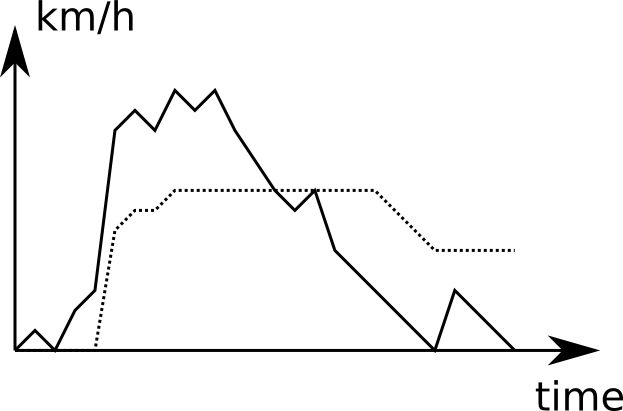
\includegraphics[width=0.4\textwidth]{../images/acckm.png}
\caption{Acckm}
\label{fig:acckm}
\end{figure}

\begin{figure}
\centering
\includegraphics[width=0.5\textwidth]{../src/images/acckmTrips.png}
\caption{Acceleration kilometers}
\label{fig:acckmTrips}
\end{figure}

\subsection{Stop and go}
Stop and go behaviour is not fuel efficient as more fuel is consumed when accelerating than when driving at a constant speed.
It is therefore interesting to see if the number of times a vehicle stops and drives on is correlated with km/l.
We say a vehicle is stopped when it decelerations below 10 km/h and that it drives again when it accelerates up above 15 km/h.
TODO: Explain why.

%TODO: Experiments

Figure~\ref{fig:stopngoTrips} shows the number of stop-and-goes of each trip normalised with the length of that trip versus the km/l of the trip.
The size of the plot indicates the amount of fuel used in the trip and the color signals what class it has been asigned to.
We see that the trips in the \fuelHigh class have few stop and goes and about half of the trips in the \fuelMedium class have more stop and goes.

\begin{figure}
\centering
\includegraphics[width=0.5\textwidth]{../src/images/stopngoTrips.png}
\caption{Number of stop and goes}
\label{fig:stopngoTrips}
\end{figure}
